\begin{columns}
  \begin{column}{0.17\linewidth}
    
\includegraphics[width=0.5\linewidth]{kth_cmyk.eps}
    \hfill
  \end{column}
  \hfill
  \begin{column}{0.64\linewidth}
    \begin{center}
      \Huge\bfseries
      From grassroots to CROCUS:\\[-0.25em]
      privacy-preserving CROwd Counting Using Smartphones
    \end{center}
    \vspace{0.25em}
    \begin{center}
      \large
      Daniel Bosk <dbosk@kth.se>
      $\bullet$
      Sonja Buchegger
      $\bullet$
      Sébastien Gambs
    \end{center}
    \vspace{1.5em}
  \end{column}
  \hfill
  \begin{column}{0.17\linewidth}
    \hfill
    
\includegraphics[width=0.8\linewidth]{uqam.pdf}
  \end{column}
\end{columns}

\vfill

\includegraphics[width=\linewidth]{ProtestVerif.png}

\vfill

\begin{columns}[t]

  \begin{column}{0.32\linewidth}

    \begin{redblock}{Verifying protest participation}
      \begin{itemize}
        \item Alice wants to show that many support her cause.
        \item Eve wants to show that few support Alice's cause.
        \item {\color{red} Adversarial setting, requires verifiable results!}
          (E.g.\ \cref{TrumpInauguration}.)
      \end{itemize}
    \end{redblock}

    \begin{blueblock}{Requirements for verifiability}
      \begin{itemize}
        \item\label{EligibilityVerif} Eligibility: anyone can verify that each 
          participation proof provides temporal and spatial eligibility and that 
          it has not been counted before.

        \item\label{UniversalVerif} Universal verifiability: anyone can verify 
          that the result is according to the submitted participation proofs.

        \item\label{IndividualVerif} Individual verifiability: every participant 
          can verify that their participation proof is included in the global 
          count.
      \end{itemize}
    \end{blueblock}

    \begin{blueblock}{Requirements for privacy}
      \begin{itemize}
        \item Protocol should not harm the privacy of the protester, i.e.\  not 
          diclose any information about them other than what can already be 
          learnt from their physical attendance.
      \end{itemize}
    \end{blueblock}

  \end{column}

  \hfill

  \begin{column}{0.32\linewidth}

    \begin{figure}
      \centering
      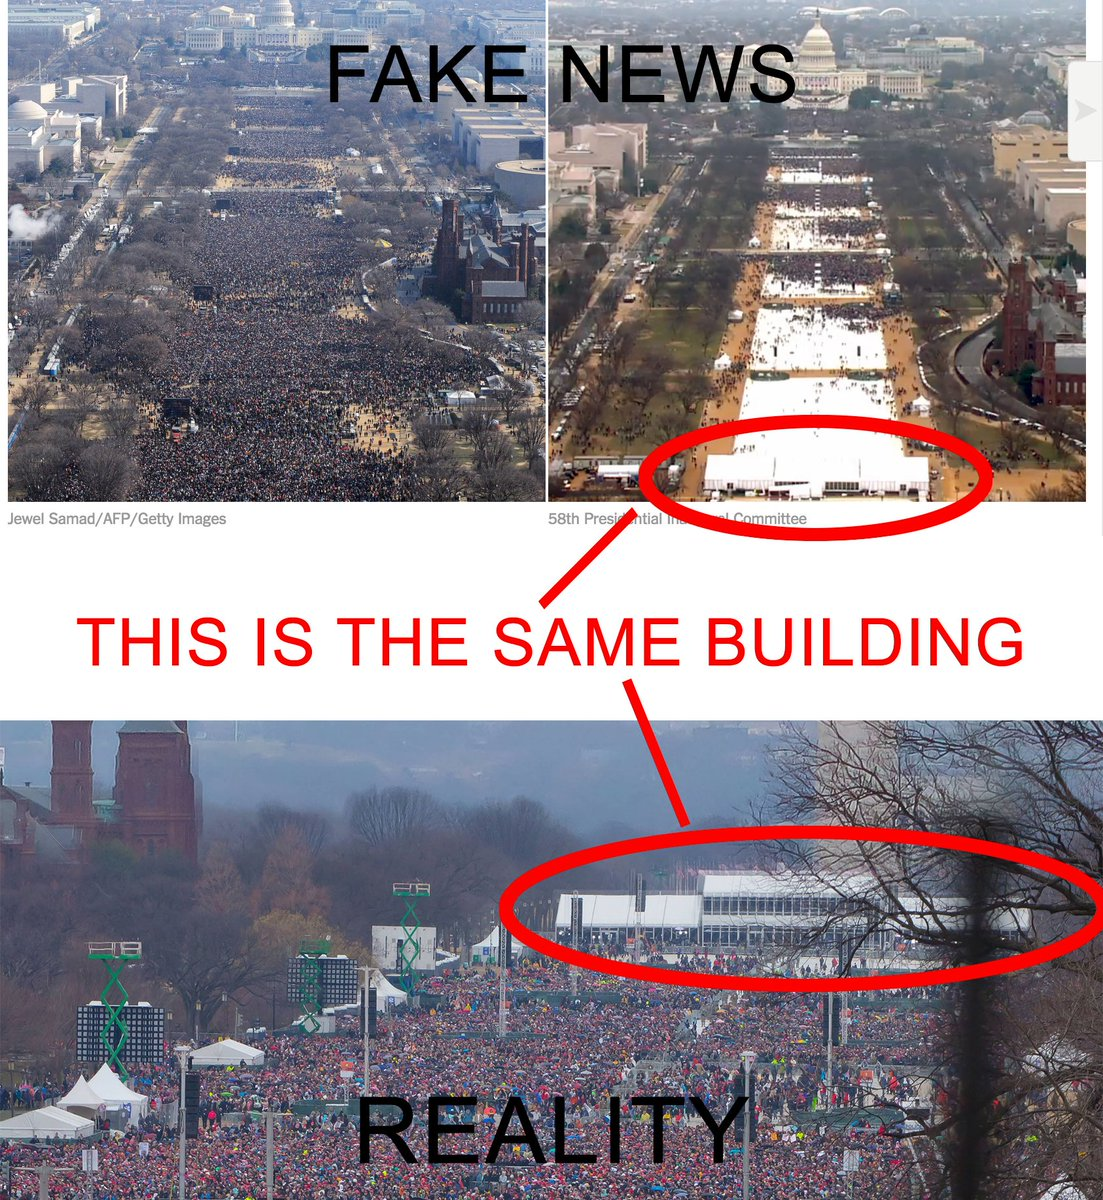
\includegraphics[width=0.9\linewidth]{trump.jpg}
      \caption{%
        What can we trust?
        This picture was posted on Twitter (and linked from Reddit) to argue 
        that the news reporting on the participation count was \enquote{fake 
          news} and that Trump's supporters arrived later.
        Even if the picture labelled \enquote{REALITY} would be from the same 
        event (difficult to verify), it is difficult to accurately compare due 
        to the angle.
        Image: Reddit/The\_Donald, Twitter.
      }\label{TrumpInauguration}
    \end{figure}

  \end{column}

  \hfill

  \begin{column}{0.32\linewidth}

    \begin{greenblock}{Our approach}
      \begin{itemize}
        \item Provides a \emph{lower bound} of the participation count.
        \item This lower bound is cryptographically verifiable.
        \item Provides privacy based on anonymous credentials and 
          privacy-preserving proximity testing.
        \item Requires only local connectivity during the protest.
        \item Requires no trust in the source (as in \cref{TrumpInauguration}), 
          only that IDs are issued correctly.
      \end{itemize}
    \end{greenblock}

    \includegraphics[width=\linewidth]{ProtestVerif-UN.png}

  \end{column}

\end{columns}

\vfill

\begin{columns}[t]

  \begin{column}{0.32\linewidth}

    \begin{figure}
      \centering
      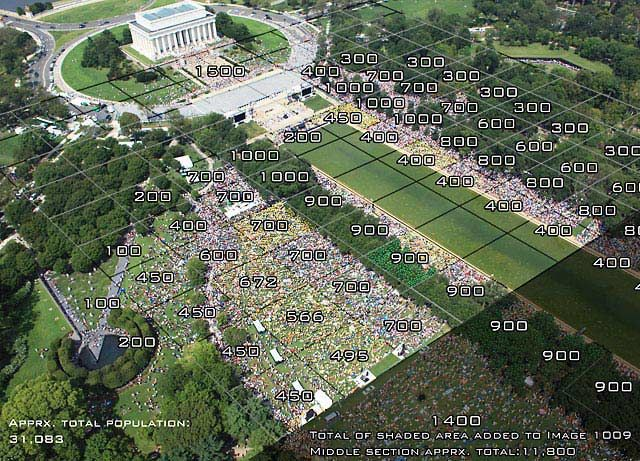
\includegraphics[width=\linewidth]{Jacobs-method.jpg}
      \caption{%
        Jacobs Method, currently most used method.
        Divide into regions, estimate density in each region, sum up.
        Image: popularmechanics.com
      }\label{JacobsMethod}
    \end{figure}

    \begin{purpleblock}{Current crowd-counting methods}
      \begin{itemize}
        \item Most used method, Jacobs Method (\cref{JacobsMethod}).
        \item {\color{red} Cannot handle cumulative counts, faces problems 
            illustrated by \cref{TrumpInauguration}.}
        \item Computer vision does object recognition; requires photos/video 
          that cover the entire location, all the time.
        \item {\color{red} This will still count people twice.}
        \item Scan active mobile phones (or similar) in the area.
        \item This requires some extra equipment.
        \item {\color{red} This catches bystanders who are not protesting.}
        \item {\color{red} Neither method can distinguish two close but 
            different protests (e.g.\ pro- and anti-protests).}
      \end{itemize}
    \end{purpleblock}

%    \begin{block}{More info}
%      \centering
%      \includegraphics[width=0.4\linewidth]{qr.eps}
%    \end{block}

  \end{column}

  \hfill

  \begin{column}{0.32\linewidth}

    \begin{blackblock}{Our scheme, during protest (\cref{ProofShare}, top of 
        \cref{Protocol})}
      \begin{itemize}
        \item The organizer publishes the protest's manifesto.
        \item Each protester reads it, approves it, computes a protest (cause) 
          identifier (\(\cid\)) to designate which protest they participate in.
        \item Each protester computes a personal identifier (\(\pid\)), 
          unlinkable between protests,
        \item Each protester acts as witness (\(\wid\), unlinkable between 
          protesters) for other protesters by creating participation-proof 
          shares.
        \item Proof shares vouches for temporal and spatial eligibility.
      \end{itemize}
    \end{blackblock}

    \begin{figure}
      \centering
      \includegraphics[width=\linewidth]{proofshare.tikz}
      \caption{\label{ProofShare}%
        Structure of a proof share.
        The protest (cause) identifier \(\cid\) is the hash value of the manifesto.
        The protester \(P\)'s identifier \(\pid\) is computed using the 
        protester's key \(\sk_P\) and \(\cid\).
        The witness \(W\)'s identifier \(\wid\) is computed using the witness's 
        key \(\sk_W\) and \(\pid\).
        \(t_s, t_s'\) are the last heads of the blockchain seen by the 
        protester and witness, respectively, and \(l\) is an area.
        All values are signed by the witness while also proving the correctness 
        of \(\wid\) and knowledge of a signature on \(\sk_W\).
      }%
    \end{figure}%

    \printbibliography[heading=none]

  \end{column}

  \hfill

  \begin{column}{0.32\linewidth}

    \begin{blackblock}{Our scheme, after the protest (bottom of 
        \cref{Protocol})}
      \begin{itemize}
        \item Proof shares are committed to a blockchain as soon as possible.
        \item \Ac{NIZK} proofs of correctness (\(\prf_\pid, \prf_\wid\) in 
          \cref{Protocol}) of \(\ACprf\) computations and knwoledge of a valid 
          signature on the key are submitted whenever convenient.
        \item Anyone can verify the proofs: eligibility, universal and 
          individual verifiability.
        \item Must be done for all shares and their \ac{NIZK} proofs.
        \item Count all \(\pid\)s with valid proofs.
      \end{itemize}
    \end{blackblock}

    \begin{figure}
      \centering
      \begin{minipage}{\linewidth}
        \begin{align*}
          O\to \text{all}\colon & \text{manifesto} \\
          P\colon & t_s\gets \TSget \\
          & \cid\gets \Hash[\text{manifesto}], \\
          & \pid\gets \ACprf[_{\sk_P}][\cid] \\
          W\colon & t_s'\gets \TSget
          \\[-1em]
          \noalign{\hfill Join}
          \midrule
          \noalign{\hfill Participation}
          \\[-3em]
          P\to W\colon & \pid \\
          P\leftrightarrow W\colon &
          \PPK\mleft\{ (\sk_P) : \mright. \\
          & \qquad \pid = \ACprf[_{\sk_P}][\cid], \\
          & \qquad \mleft. \sigma_P' = \ACblind[\ACsign[_{\ssk}][\sk_P]] \mright\} 
          \\
          W\colon & \wid\gets \ACprf[_{\sk_W}][\pid] \\
          W\to P\colon & (\wid, t_s', l)
          \\[-1em]
          \noalign{\hfill Participation}
          \midrule
          \noalign{\hfill Submission}
          \\[-2em]
          P\colon & t_e\gets \TSstamp[\Hash[\pid, \wid, t_s, t_s', l]] \\
          W\colon & t_e'\gets \TSstamp[\Hash[\pid, \wid, t_s, t_s', l]] \\
          W\to S\colon & (\pid, \wid, t_s, t_s', t_e, l, \pi_{\wid}),\quad 
          \text{where} \\
          & \pi_{\wid} = \SPK\mleft\{ (\sk_W) : \mright. \\
          & \qquad \wid = \ACprf[_{\sk_W}][\pid], \\
          & \qquad \mleft. \sigma_W' = \ACblind[\ACsign[_{\ssk}][\sk_W]]\mright\} 
          \\
          & \qquad\qquad (\pid, \wid, t_s, t_s', l) \\
          P\to S\colon & (\cid, \pid, \wid, t_s, t_s', t_e, l, \pi_{\pid}),\quad 
          \text{where}\\
          & \pi_{\pid} = \SPK\mleft\{ (\sk_P) : \mright. \\
          & \qquad \pid = \ACprf[_{\sk_P}][\cid], \\
          & \qquad \mleft. \sigma_P' = \ACblind[\ACsign[_{\ssk}][\sk_P]] \mright\} 
          \\
          & \qquad\qquad (\cid, \pid, \wid, t_s, t_s', l)
        \end{align*}
      \end{minipage}
      \caption{\label{Protocol}%
        An overview of the Join, Participation and Submission phases of \CROCUS.\@
        The organizer \(O\) broadcasts the manifesto.
        The protester \(P\), witness \(W\) and their computations are as in 
        \cref{ProofShare}.
        Finally, both \(P\) and \(W\) submits the proof shares to a permanent storage \(S\).
      }%
    \end{figure}

  \end{column}

\end{columns}

\vfill
\flushright{}
Special thanks to xkcd.com which, over many years, has inspired the stylistic 
presentation of this poster.
